\documentclass[a4paper,12pt]{article}

\usepackage[T1]{fontenc}
\usepackage[utf8]{inputenc}
\usepackage[english, polish]{babel}
\usepackage{lmodern}
\usepackage{graphicx}
\usepackage{fancyhdr}
\usepackage{float}
\usepackage{array}
\usepackage{hyperref}
%\usepackage{mathtools}


\setlength{\textheight}{23.5cm}
\setlength{\textwidth}{15.92cm}
\setlength{\footskip}{10mm		}
\setlength{\oddsidemargin}{0mm}
\setlength{\evensidemargin}{0mm}
\setlength{\topmargin}{0mm}
\setlength{\headsep}{15mm}
\setlength{\parindent}{0cm}
\setlength{\parskip}{2.5mm}
%nowa extra row do tabeli :)  :) 
\setlength{\extrarowheight}{4pt}

\author{Justyna Ilczuk, Jacek Rosiński}

\begin{document}

\begin{center}

    \begin{tabular}{ | m{5cm}| m{5cm} | m{5cm} |}
    \hline 
    \multicolumn{2}{|c|}{{ \Large \textbf{Laboratorium Fizyki 2}} }
    &  
    \begin{center}
    Data wykonania ćwiczenia:
    \end{center}
    \begin{center}
      16.10.2013 
    \end{center}
    \begin{center}
    Środa 9.45-12.45
    \end{center}
     \\ 
    
    \hline
    \multicolumn{2}{|c|}{Justyna Ilczuk \newline Jacek Rosiński}
    & \begin{center}
    {\small Data złożenia sprawozdania:} \newline \today
    \end{center}   \\
   	
   	\hline
    Wydział Fizyki & Grupa: K-1 \newline Rok akademicki: 2013/2014 &    Nr ćwiczenia: 6 \\
   	\hline
   	\multicolumn{2}{|l|}{Prowadzący: Piotr Panecki} & \multicolumn{1}{|l|}{Ocena końcowa:}\\
    \hline
    \end{tabular}
\end{center}

\newpage

\pagestyle{fancy}
\fancyfoot[CO]{\ }
\fancyhead[RO]{\footnotesize{\thepage} }
%\fancyhead[RO]{\footnotesize{\ } }
\fancyhead[LO]{Justyna Ilczuk i Jacek Rosiński K-1, Zjawisko tunelowe dla fal elektromagnetycznych }

% wrzucanie wykresów:

%\begin{figure} [H]
%  \begin{center}
%    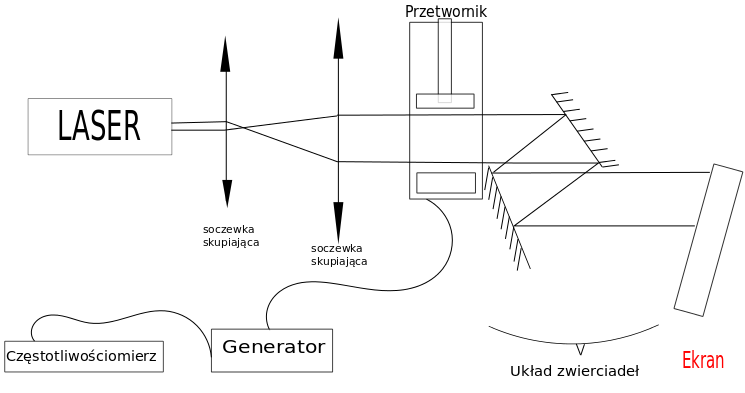
\includegraphics[width = 15cm]{Rysunek.png}
%    \caption{Układ pomiarowy}
%  \end{center}
%\end{figure}


\section{Cel ćwiczenia}

Celem ćwiczenia było zbadanie zjawiska tunelowania dla fal elektromagnetycznych. Badając przechodzenie fali Elektromagnerycznej spodziewamy się zobaczyć zmniejszanie się mocy dali wraz z odegłością, zależności $E~e^{-\gamma x}$. 

\section{Wstęp}

Fala elektromagnetyczna ulega zjawisku całkowitego wewnętrznego odbcia - zależność $\frac{n_1}{n_2}\cdot \sin \theta_gr = 1 $. Zanikanie wiązki światła na granicy dwóch ośrodków, nie oznacza że pole elektryczne i magnetyczne fali elektromagnetycznej zanika w sposób skokowy na granicy dwóch ośrodków. Te pola wnikają na pewną głębokość do obszary, w którym fala elektromagnetyczna się nie propaguje. 
%u są wzory których nie rozumiem więc ich nie zżynam 
Jeśli jednak grubość warstwy w której pole zanika jest mała, a za nią znajduje się obszar, w którym fala elektromagnetyczna może się rozprzestrzeniać, to jej część przejdzie do tego obszaru, co określamy jako \textbf{efekt tunelowy} określony zależnością.


$$
E = E_0cos(wt-k_{II}y)e^{-\gamma x} \\
$$
$$
\gamma = n_2k_0
$$

\section{Użyty sprzęt i układy pomiarowe}

Do przeprowadzenia eksperymentu używaliśmy: 

\begin{enumerate}
  \item Modulatora fal EM (mikrofalowych, centymetrowych) 
  \item Miernika uniwersalnego Metatronik V640 połączonego z odniornikiem fal elektromagnetycznych
  \item Miarki z podziałką milimetrową do przesuwania substancji o wysokim współczynniku załamania  (pryzmatów parafinowych)
  
\end{enumerate}


\section{Opracowanie wyników}

Wyniki pomiarów przedstawiamy poniżej w tabelce:

Pomiary odbitej wiązki:

\begin{tabular}{ l | c | r }
  		x [cm] & V [mV] & zakres [mV] \\
  		\hline
		18&127&150 \\
		16.5&123&150 \\
		15&119&150 \\
		13&115&150 \\
		12.2&105&150 \\
		11.8&95&150 \\
		11.3&80&150 \\
		11&63&150 \\
		10.8&42&150 \\
		10.5&23&50 \\
		10.3&15&50 \\
		9.9&3.3&5 \\


\end{tabular}

Pomiary wiązki, która przetunelowała:

\begin{tabular}{ l | c | r }

	x [cm] & V [mV] & zakres [mV] \\
	\hline
	10.3&105&150 \\
	10.7&87&150 \\
	11&71&150 \\
	11.2&55&150 \\
	11.4&46&150 \\
	11.6&36&50 \\
	12&25&50 \\
	12.3&19&50 \\
	12.8&9&50 \\
	13.4&4.5&15 \\
	13.8&3.3&5 \\
	14.5&1.7&5 \\
	15&0.9&1.5 \\
	16.4&0.5&1.5 \\

\end{tabular}



\begin{figure} [H]
  \begin{center}
    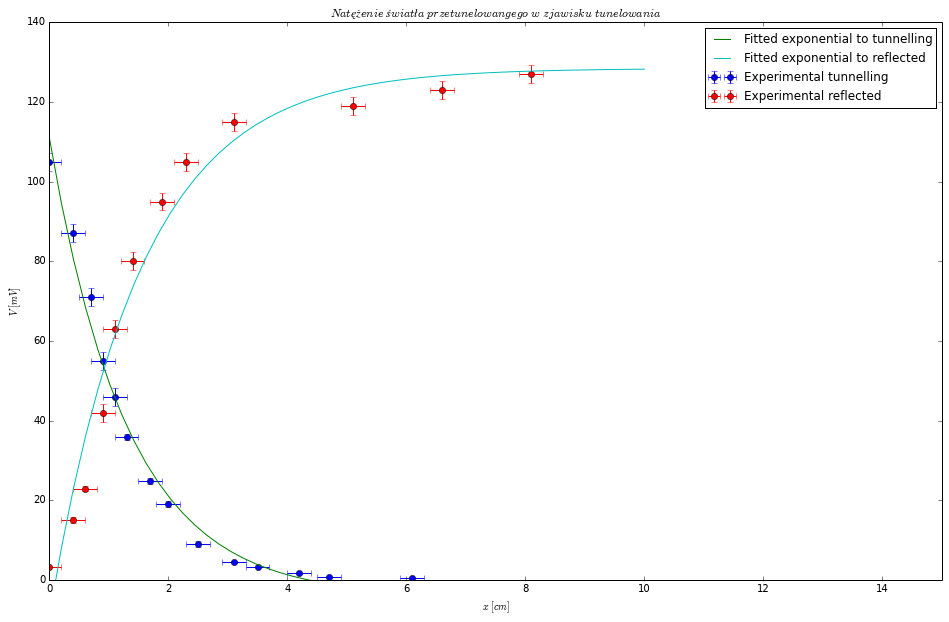
\includegraphics[width = 15cm]{prettier_plot.png}
    \caption{Zmierzone natężenia fal od przerwy między ośrodkami}
  \end{center}
\end{figure}

Dopasowaliśmy krzywe wykładnicze metodą najmniejszych kwadratów, używając do tego biblioteki do obliczeń naukowych 

\href{'http://docs.scipy.org/doc/scipy/reference/tutorial/optimize.html'}{scipy.optimize}


$y = a e^{-bx} + c$

$a = 115.42$

$b = 0.76$

$c = -4.27 $


Macierz kowariancji otrzymanych współczynników:

\begin{center}

    \begin{tabular}{ | m{5cm}| m{5cm} | m{5cm} |} \hline
    
    
    1.46e+01  &   7.76e-03 & -4.45e+00 \\ \hline

 	7.76e-03  & 3.69e-03  & 1.29e-01 \\ \hline
    
    -4.45e+00 &  1.28e-01 &  7.23e+00 \\ \hline
    \end{tabular}
\end{center}


niestety wyliczone przez nas $\chi^2$ zredukowane miało wartość ok. 3000. Analizując nasze pomiary i wyniki, doszliśmy do wniosku, że tak wysoką wartość $\chi^2$ uzyskaliśmy przez zaniżenie niepewności pomiarowych w naszym doświadczeniu.


<<<<<<< Updated upstream
=======
W doświadczeniu również otrzymaliśmy szansę zmierzenia długości fali. W tm celu Użyliśmy płytki z otworami, które były co ok 1 cm. Płytka ustawiona w sposób blokujący przepuszczała część promieniowania, wiec nei mżna jej było nazwać polaryzatorem, a jedynei płytką półprzepuszczalną. Na podstawie tej właściwości przeprowadziliśmy dwa eksperymenty (zmiana odległości płytki półprzepuszczalnej i interferometr Michelsona) z których wynikało ze długość fali wynosi $ 1: \lambda= 3,2 (0,3) cm  $, $ \lambda= 3,1 (0,3) cm $.


>>>>>>> Stashed changes
\section{Wnioski}

Jacek, weź uzupełnij to twoimi wnioskami, które były na wydruku, ok? I popraw tam błędy ortograficzne.

%{\Large Hipoteza potwierdzona, ta fizyka jest szalona! }

W doświadczeniu zaobserwowano tunelowanie fali elektromagnetycznej, której moc spada eksponencjalnie wraz ze odległością ośrodków rozchodzenia się fali. 
Fala mikrofalowa jakiej używaliśmy miała długość około 	3.2 cm.


%\section {Źródła dodatkowe}
  
 %kosmos i obserwacja losowych zachować w koloniach mrówek. 

\end{document}
